\chapter{Introduzione} \label{chap:introduction}

\section{Evoluzione dell'astrofotografia} \label{sec:evolution}

L'\textbf{\href{https://it.wikipedia.org/wiki/Astrofotografia}{astrofotografia}} si occupa di fotografare oggetti celesti come stelle, pianeti, galassie e nebulose. Questa pratica ha radici risalenti al XIX secolo: nel 1822 fu scattata la prima foto nella storia da Nicéphore Niépce, e già nel 1840 John William Draper catturò la prima immagine della Luna, segnando l'inizio di una nuova era nell'osservazione astronomica. Nel 1850, William Cranch Bond e John Adams Whipple scattarono la prima fotografia di una stella, \textit{Vega}, con un'esposizione di 1000 secondi.

\subsection{Breve storia e sviluppo tecnologico} \label{subsec:history}

Nei primi anni le immagini erano ottenute con \textit{lastre fotografiche di vetro}, che richiedevano tempi di esposizione estremamente lunghi. Catturare immagini di oggetti deboli come nebulose e galassie era un'impresa ardua e poteva richiedere ore o notti intere di esposizione, rendendo il processo molto laborioso. Le prime immagini si concentravano infatti su oggetti luminosi, come la Luna e i pianeti, mentre stelle più deboli e galassie rimanevano al di là delle capacità tecnologiche dell'epoca \cite{astroph_hist}. 
Con la nascita della \textit{fotografia a colori} gli astronomi potettero registrare le diverse tonalità di colore degli oggetti celesti, rendendo possibile ottenere informazioni circa la composizione chimica e la temperatura di stelle e nebulose. La vera rivoluzione arrivò con l'avvento della \textbf{\href{https://it.wikipedia.org/wiki/Fotografia_digitale}{fotografia digitale}} e l'introduzione di \textit{dispositivi a carica accoppiata} (\textit{CCD}) alla fine degli anni '60. I \textit{CCD} avevano sensibilità alla luce notevolmente superiore rispetto alle lastre fotografiche, permettendo tempi di esposizione più brevi e maggiore qualità dell'immagine. Ciò consentì di rilevare oggetti celesti più deboli e ridurre significativamente il rumore nelle immagini \cite{multiwavelength_image_proc}.

Con la diffusione dei computer, l'elaborazione delle immagini digitali divenne parte integrante dell'astrofotografia. Tecniche come la \textit{calibrazione}, l'\textit{allineamento}, la \textit{riduzione del rumore} e lo \textit{stacking} delle immagini hanno permesso di ottenere risultati di qualità superiore rispetto alle immagini singole. L'utilizzo di algoritmi avanzati consentì di rivelare dettagli nascosti, migliorare il  contrasto e ridurre al minimo il rumore aumentando l'accuratezza delle osservazioni astronomiche \cite{calibration_1}\cite{calibration_2}.

Oggi l'astrofotografia è accessibile non solo ad astronomi professionisti, ma anche ad appassionati dilettanti. L'ampia disponibilità di telescopi, fotocamere e software avanzati ha reso possibile catturare immagini di alta qualità anche con strumenti di costo contenuto. L'astrofotografia è diventata un hobby popolare tra appassionati di astronomia e fotografia, che condividono le proprie immagini e scoperte sui social e forum online come \textit{\href{https://www.cloudynights.com/index}{Cloudy Nights}} o \textit{\href{https://www.astrobin.com}{AstroBin}}.

\section{Stato dell'arte: strumentazione e tecniche moderne} \label{state_of_the_art}

L'astrofotografia moderna si avvale di strumenti sofisticati e tecniche avanzate per catturare immagini di alta qualità. I telescopi sono dotati di montature motorizzate che compensano il movimento apparente del cielo, consentendo esposizioni più lunghe senza sfocature. Le fotocamere digitali, spesso equipaggiate con sensori \textit{CCD} o \textit{CMOS}, sono in grado di catturare immagini ad alta risoluzione anche di oggetti celesti deboli quali galassie o nebulose, preservandone i dettagli. I software di elaborazione delle immagini offrono strumenti avanzati per la calibrazione, l'allineamento e la post-produzione delle immagini, consentendo di ottenere risultati di qualità professionale.

\begin{figure}[h]
    \centering
    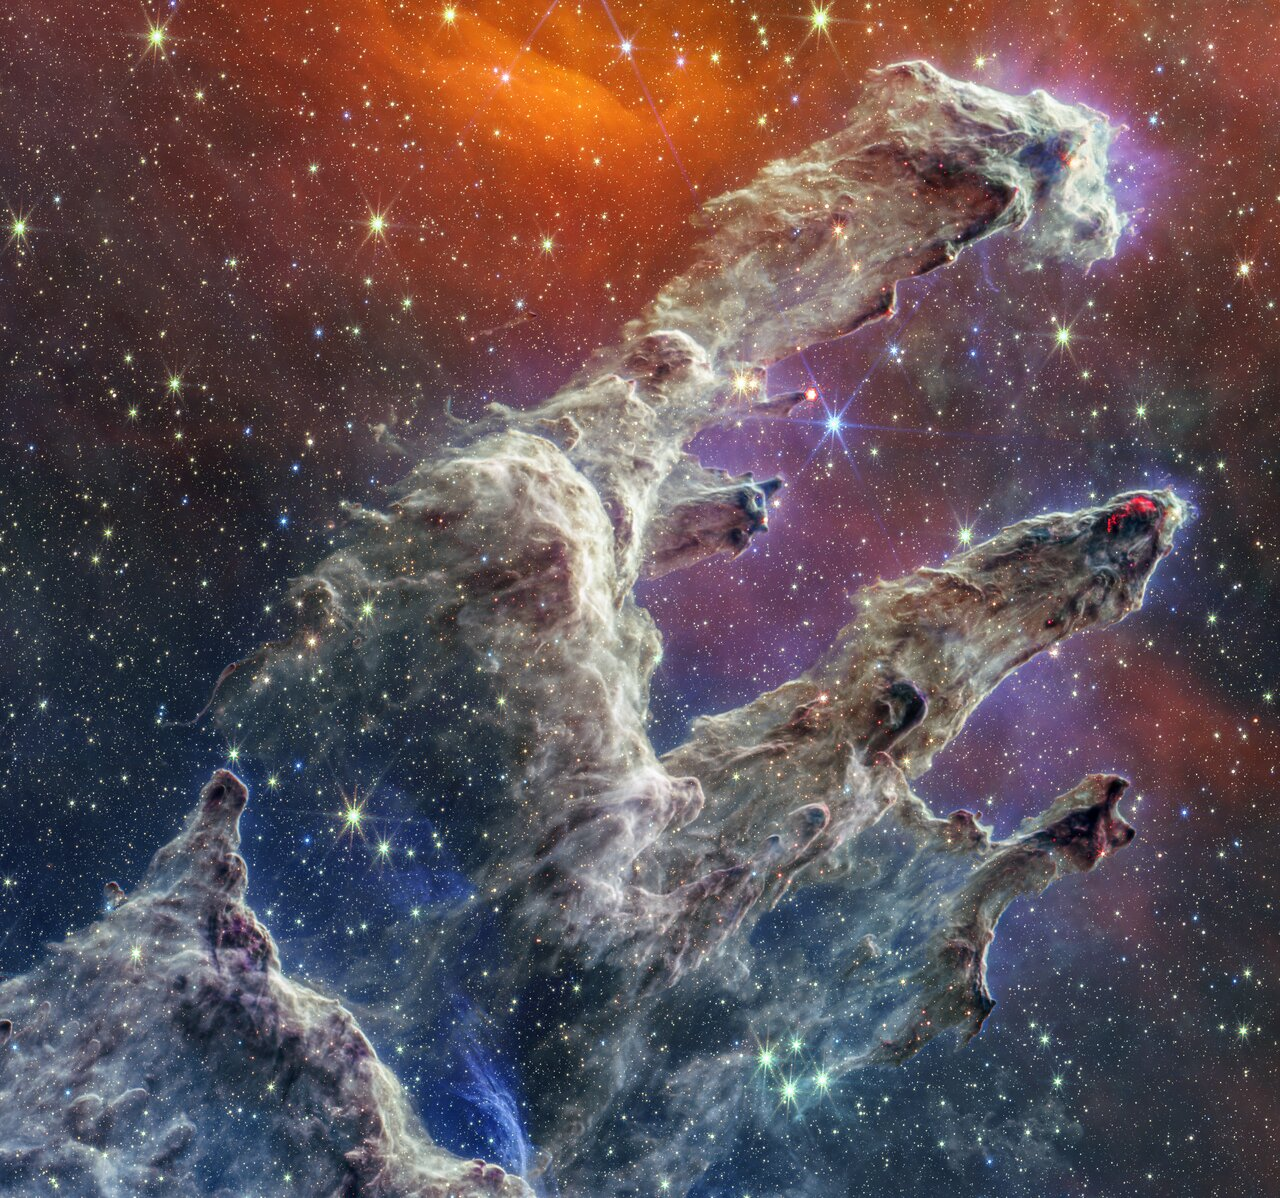
\includegraphics[scale = 0.6]{../assets/Webb_POC.jpg}
    \captionsetup{justification=centering}
    \caption{\textit{Pillars of Creation}, \textit{Nebulosa dell'Aquila}, ripresi dal \textit{James Webb} combinando dati acquisiti da \textit{NIRCam} e \textit{MIRI}. Immagine originale su \href{https://webbtelescope.org/contents/media/images/01GK2KKTR81SGYF24YBGYG7TAP}{webbtelescope.org}} \label{fig:webb_poc}
\end{figure}

Esistono diversi telescopi spaziali, come l'\textit{\href{https://hubblesite.org/home}{Hubble Space Telescope}} \cite{hubble} della \textit{NASA} e il \textit{\href{https://webbtelescope.org/home}{James Webb Space Telescope}} \cite{jwst}, gestito congiuntamente da \textit{ESA}, \textit{NASA} e \textit{CSA}. Questi strumenti, orbitando al di fuori dell'atmosfera terrestre, sono in grado di catturare immagini ad altissima risoluzione e sensibilità, libere dalle distorsioni e dall'inquinamento luminoso terrestre. Sfruttano a proprio vantaggio fenomeni fisici come le \textit{lenti gravitazionali} e la \textit{diffrazione} per osservare oggetti nello spazio profondo, ben oltre le capacità degli strumenti terrestri. Questi telescopi, inoltre, sono dotati di telecamere come la \textit{NIRCam} (Near Infrared Camera) e la \textit{MIRI} (Mid Infrared Instrument), che permettono di osservare l'universo in bande di luce altrimenti invisibili, rivelando dettagli nascosti e processi fisici altrimenti inaccessibili (\cref{fig:webb_poc}), e si dimostrano fondamentali per la ricerca astronomica.

\subsection{Hardware} \label{subsec:hardware}

Nell'astrofotografia tradizionale si utilizzano principalmente tre tipi di strumenti:

\begin{itemize}
    \item \textbf{Telescopi}: I telescopi sono fondamentali nell'astrofotografia; ne esistono di diversi tipi, tra cui rifrattori, riflettori e catadiottrici, ciascuno con caratteristiche specifiche. I telescopi moderni variano da piccoli modelli portatili a grandi strutture professionali, come l'\textit{\href{https://elt.eso.org/}{ELT}} (Extremely Large Telescope), con uno specchio principale di ben $ 39 \text{m} $ di diametro, che è ancora in costruzione ma si prevede diventerà operativo entro il 2027 \cite{elt}. La scelta del telescopio dipende dall'oggetto celeste da osservare e dal livello di dettaglio desiderato, oltre che dal budget disponibile.

    \item \textbf{Fotocamere}: Le fotocamere \textit{\textbf{CCD}} (Charge-Coupled Device) sono ampiamente utilizzate in ambito astronomico per la loro alta sensibilità e basso \hyperref[sec:noise]{rumore elettronico}. Negli ultimi anni, le fotocamere \textit{\textbf{CMOS}} (Complementary Metal-Oxide-Semiconductor) hanno guadagnato popolarità in quanto più performanti e più accessibili economicamente. Tali fotocamere offrono elevate risoluzioni, velocità di lettura più rapide e buona \href{https://it.wikipedia.org/wiki/Efficienza_quantica}{\textit{efficienza quantica}}, rendendole adatte sia per l'uso professionale che amatoriale \cite{image_processing}.
    
    \item \textbf{Montature}: Una montatura stabile e precisa è essenziale per compensare la rotazione terrestre durante le lunghe esposizioni.

    \begin{itemize}
        \item Le \textit{montature equatoriali} sono progettate per seguire il movimento apparente delle stelle nel cielo, consentendo di mantenere gli oggetti celesti centrati nell'inquadratura.
        \item Le \textit{montature altazimutali}, più semplici da utilizzare, richiedono sistemi di derotazione o software di correzione più sofisticati per lunghe esposizioni, a causa della rotazione di campo.
        \item Le \textit{montature computerizzate}, dotate di sistemi \textit{GoTo}, permettono di puntare automaticamente verso specifici oggetti celesti e di tracciarli con precisione.
    \end{itemize}

\end{itemize}

\subsection{Software e algoritmi nell'astrofotografia} \label{subsec:software}

Con il tempo i software utilizzati in ambito astrofotografico sono arrivati al punto tale per cui non è necessario essere dotati di un \hyperref[subsec:hardware]{hardware} professionale per catturare immagini di corpi celesti anche dal proprio cortile (o \textit{"from my backyard"}).

I software principalmente utilizzati, quali \href{https://pixinsight.com/}{\textit{PixInsight}} o \href{https://www.autostakkert.com/}{\textit{AutoStakkert}} implementano diversi algoritmi in grado di migliorare sensibilmente i risultati finali:

\begin{itemize}
\item \textbf{Calibrazione delle immagini}: La calibrazione è un passaggio cruciale per rimuovere artefatti e rumori dovuti alla strumentazione dalle immagini astronomiche. Questo processo utilizza diversi insiemi di frame di calibrazione: \textit{bias frames, dark frames} e \textit{flat frames} (più nel dettaglio nella \cref{sec:calibration}) dai quali è possibile estrarre informazioni sul rumore dell'immagine, così da poterlo sottrarre alla stessa \cite{calibration_1} \cite{calibration_2}.

\item \textbf{Allineamento delle immagini}: L'allineamento è necessario per combinare correttamente più immagini dello stesso oggetto. Algoritmi di feature detection come \textit{\textbf{ORB}} (Oriented FAST and Rotated BRIEF) \cite{orb}, \textit{\textbf{SIFT}} (Scale-Invariant Feature Transform) e \textit{\textbf{SURF}} (Speeded Up Robust Features) identificano punti caratteristici nelle immagini per calcolare \hyperref[subsec:homography]{\textit{trasformazioni omografiche}}, utilizzate per correggere differenze di scala, rotazione e prospettiva tra le immagini (più nel dettaglio nella \cref{sec:alignment}) \cite{multiwavelength_image_proc} \cite{calibration_2}.

\item \textbf{Riduzione del rumore}: La riduzione del rumore migliora la qualità finale delle immagini. Tecniche tradizionali come l'unsharp masking \cite{multiwavelength_image_proc} accentuano i dettagli sottraendo una versione sfocata dell'immagine originale. Approcci più avanzati utilizzano reti neurali convoluzionali profonde, come \textit{\textbf{DnCNN}} (Denoising Convolutional Neural Network) \cite{DnCnn}, che apprendono a rimuovere il rumore preservando i dettagli attraverso l'addestramento su grandi dataset (più nel dettaglio nelle sezioni \ref{sec:preprocessing} e \ref{sec:postprocess}).

\item \textbf{Stacking delle immagini}: Lo \textit{stacking} (\textit{"impilamento"}) combina multiple esposizioni per ottenere un'unica immagine finale ottimizzandone il rapporto segnale-rumore. Questa tecnica riduce il rumore casuale e mette in evidenza dettagli deboli non visibili in singole esposizioni. Metodi come il \textbf{\textit{Weighted Average Stacking}} assegnano un peso a ciascuna immagine in base ad un criterio prefissato, per ottenere in seguito un'immagine data dalla media ponderata dei valori dei singoli frames in input (più nel dettaglio nella \cref{sec:stacking}).
\end{itemize}

\section{Rumori e artefatti nelle immagini astronomiche} \label{sec:noise}

La qualità delle immagini astronomiche è influenzata da diversi tipi di rumore e artefatti, che devono essere mitigati per ottenere risultati ottimali:

\begin{itemize}
    \item \textbf{Rumore termico}: Il rumore termico (\textit{Dark Current}) è generato dall'agitazione termica degli elettroni all'interno del sensore della fotocamera, producendo un segnale anche in assenza di luce. Questo tipo di rumore aumenta con la temperatura del sensore ed è particolarmente significativo nelle lunghe esposizioni. Per ridurlo, molti sensori astronomici sono raffreddati tramite \textit{sistemi termoelettrici} o \textit{criogenici}. La sottrazione dei \hyperref[subsec:dark]{\textit{dark frames}} durante la calibrazione permette di correggere questo rumore.
    
    \item \textbf{Rumore del sensore}: Include diversi tipi di rumore intrinseco al sensore della fotocamra:
    
    \begin{itemize}
        \item \textbf{Rumore di lettura}: deriva dall'elettronica durante il processo di lettura e digitalizzazione del segnale dal sensore. È generalmente costante e può essere minimizzato utilizzando componenti elettronici di alta qualità. Sebbene il rumore di lettura non possa essere eliminato, l'uso di \hyperref[subsec:bias]{\textit{bias frames}} nella calibrazione aiuta a compensare l'offset introdotto dall'elettronica.
        
        \item \textbf{Rumore di schema fisso}: Il rumore di schema fisso (\textit{Fixed Pattern Noise}) è causato dalle variazioni di sensibilità tra i pixel, si manifesta come pattern ripetuti nell'immagine. L'utilizzo dei \hyperref[subsec:flat]{\textit{flat frames}} nella calibrazione aiuta a correggere queste imperfezioni.
        
        \item \textbf{Amp glow}: È una luminescenza causata dal calore generato dai circuiti di amplificazione del sensore, visibile come un bagliore ai bordi dell'immagine. La sottrazione dei \hyperref[subsec:dark]{\textit{dark frames}} e il raffreddamento del sensore contribuiscono a ridurre questo fenomeno.
    \end{itemize}
    
    \item \textbf{Altri artefatti}: altri artefatti includono la vignettatura, un oscuramento ai bordi dell'immagine dovuto alle caratteristiche ottiche del sistema e mitigabile con i \hyperref[subsec:flat]{\textit{flat frames}}, e i \textit{pixel caldi e morti},  ossia pixel che rimangono sempre accesi o spenti, che possono essere mappati e corretti durante l'elaborazione.

\end{itemize}

\section{La Luna} \label{sec:moon}

Tra i corpi celesti più affascinanti e accessibili nell'astrofotografia spicca sicuramente la \textbf{Luna}. Grazie alla sua vicinanza alla Terra, alla sua luminosità e alle sue dimensioni apparenti relativamente grandi, è possibile catturare immagini lunari di alta qualità anche in assenza di strumentazione professionale. Fotografare la Luna rispetto ad altri corpi celesti presenta diversi vantaggi:

\begin{itemize}
    \item \textbf{Rotazione sincrona}: La Luna mostra sempre la stessa faccia verso la Terra a causa della sua \textit{rotazione sincrona}, ovvero il suo periodo di rotazione attorno al proprio asse è uguale al periodo di rivoluzione attorno alla Terra (circa 27,3 giorni) [\cref{fig:moonrota}]. Questo fenomeno, dovuto alla \textit{risonanza mareale}, comporta diverse semplificazioni nell'elaborazione delle immagini, eliminando la necessità di processi di derotazione \cite{nasa_moon_orbit}.
    
    \item \textbf{Luminosità elevata}: La Luna è l'oggetto celeste più luminoso nel cielo notturno. Questa luminosità consente di utilizzare tempi di esposizione più brevi rispetto ad altri oggetti astronomici (da $1/250$ a $1/100$ di secondo, a seconda della percentuale di illuminazione, contro tempi fino a $20$-$30$ secondi per oggetti dello spazio profondo), riducendo gli effetti del \hyperref[sec:noise]{rumore elettronico} e del movimento apparente.
    
    \item \textbf{Facilità di localizzazione}: Essendo facilmente visibile ad occhio nudo, la Luna non richiede sistemi di puntamento sofisticati o montature equatoriali per essere fotografata. Un semplice treppiede è sufficiente per stabilizzare la fotocamera durante la cattura delle immagini.
\end{itemize}

Nell'astrofotografia planetaria in generale, quando il soggetto non è la Luna, i pianeti sono notevolmente distanti dalla Terra, e piccole perturbazioni dell'atmosfera possono causare rumore e artefatti fastidiosi. È possibile ovviare a questo problema registrando dei video (piuttosto che singole immagini) e rimuovere tali artefatti tramite una tecnica chiamata \textit{Lucky Imaging}, combinata con tecniche di \textit{derotazione} per mitigare l'effetto della rotazione del pianeta attorno al proprio asse.

L'astrofotografia lunare professionale consiste spesso nello scattare immagini che catturano sezioni diverse della Luna; queste vengono prima processate singolarmente e poi unite mediante tecniche di \textit{stitching}. Un'altra tecnica molto diffusa è quella utilizzata per ottenere le cosiddette \textit{Mineral Moon}: si eseguono diversi scatti applicando filtri a banda stretta sui telescopi, per poi elaborare i canali RGB singolarmente, facendo risaltare la presenza di minerali diversi sulla superficie lunare \cite{legault_astrophoto}.

\begin{figure}
    \centering
    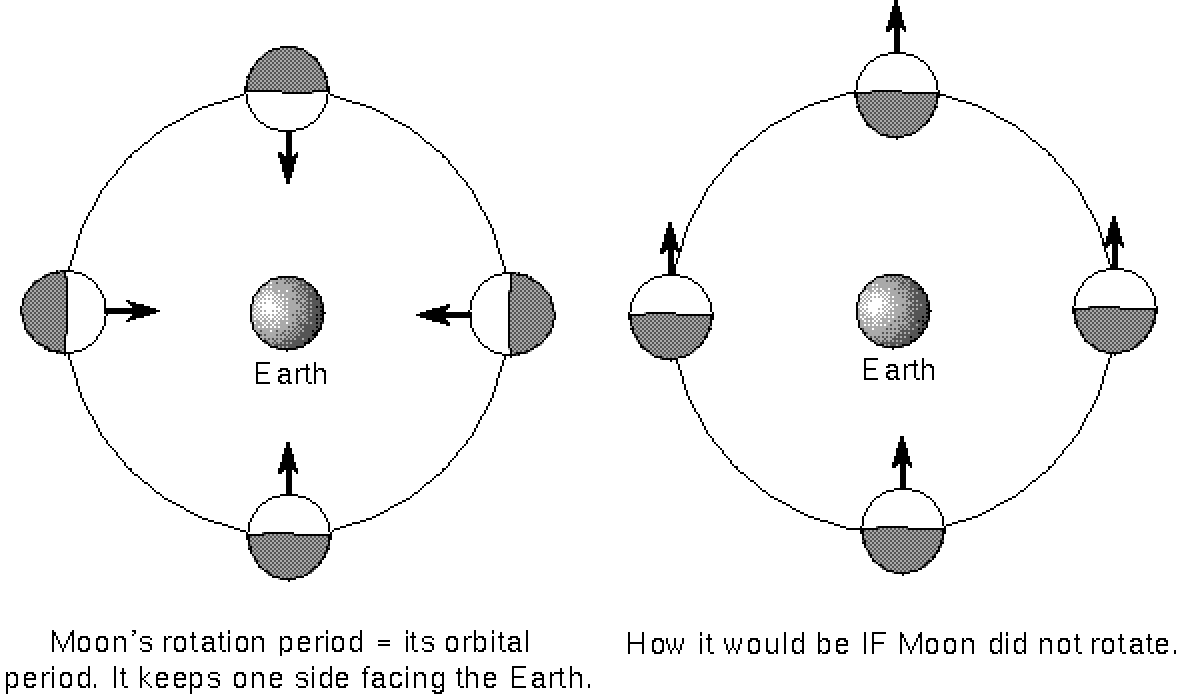
\includegraphics[scale = 0.4]{../assets/moonrota.png}
    \captionsetup{justification=centering}
    \caption{Dimostrazione grafica del moto di rotazione e rivoluzione della Luna. Questa immagine è per gentile concessione di \textit{Nick Strobel} su \href{www.astronomy\_notes.com}{www.astronomy\_notes.com}} \label{fig:moonrota}
\end{figure}

Fotografare la Luna presenta comunque diverse sfide. Essa è caratterizzata da un elevato contrasto tra le aree illuminate e quelle in ombra, specialmente durante le fasi parziali, rendendo difficile ottenere un'esposizione bilanciata che catturi dettagli in entrambe le zone \cite{sheehan_epic_moon}. Nonostante la sua vicinanza, l'atmosfera terrestre influenza la qualità delle immagini lunari, introducendo turbolenze (\textit{seeing}), dispersione e attenuazione della luce, portando ad una riduzione di nitidezza e contrasto nei risultati \cite{sheehan_epic_moon}. Infine, sebbene la luminosità della Luna consenta di fotografarla anche da aree urbane, l'inquinamento luminoso può ancora influenzare la qualità, specialmente quando si vuole catturare dettagli più fini o nelle le fasi meno illuminate.

Nel contesto di questo progetto, sono state scattate personalmente immagini della Luna utilizzando una \textbf{Fujifilm FinePix S1}, una fotocamera bridge dotata di uno zoom ottico fino a $50 \times$. Senza l'ausilio di telescopi o montature specializzate, ma semplicemente con l'utilizzo di un treppiede standard, è stato possibile catturare immagini dettagliate della superficie lunare.

Questa scelta strumentale evidenzia come, grazie alle moderne tecnologie e alle tecniche di elaborazione delle immagini, sia possibile ottenere risultati di qualità anche con attrezzature relativamente modeste. Le immagini acquisite sono state utilizzate per testare e validare gli algoritmi sviluppati nel corso del progetto, dimostrando l'efficacia delle metodologie proposte nell'ottimizzazione di fotografie lunari.
\cleardoublepage